% Macro-wired AdverSim manuscript scaffold.
% This is a presentation-fix draft: use it as the manuscript entry point or
% copy sections into the journal template. Headline numbers must come from
% paper/generated_macros.tex rather than being hard-coded.

\documentclass[conference]{IEEEtran}
\usepackage{graphicx}
\usepackage{booktabs}
\usepackage{url}

% generated_macros.tex
% DO NOT EDIT BY HAND -- produced by analysis/build_results_registry.py

\newcommand{\AttackVersionMinScenarioActive}{100.0\%}
\newcommand{\AttackVersionMinUniqueActive}{100.0\%}
\newcommand{\AttackVersionsCompleted}{3}
\newcommand{\BaseCoverage}{48.8\%}
\newcommand{\BaselineAdverSimBaseCoverage}{48.8\%}
\newcommand{\BaselineAdverSimTransition}{61.4\%}
\newcommand{\BaselineAtomicBaseCoverage}{71.1\%}
\newcommand{\BaselineAtomicUniqueActive}{320}
\newcommand{\BaselineCalderaBaseCoverage}{19.4\%}
\newcommand{\BaselineCalderaTransition}{83.6\%}
\newcommand{\BaselineCalderaUniqueActive}{47}
\newcommand{\CostPerScenario}{0.000322}
\newcommand{\DetEnvCloud}{0.671}
\newcommand{\DetEnvEnterprise}{0.649}
\newcommand{\DetEnvHealthcare}{0.649}
\newcommand{\DetEnvICS}{0.678}
\newcommand{\ExtCorrob}{55.8\%}
\newcommand{\ExtCorrobWeighted}{57.0\%}
\newcommand{\ExternalCliffDelta}{1.000}
\newcommand{\ExternalRandomMean}{0.777}
\newcommand{\ExternalRealMean}{0.977}
\newcommand{\ExternalReports}{40}
\newcommand{\FirstAttemptCIhi}{94.3\%}
\newcommand{\FirstAttemptCIlo}{91.1\%}
\newcommand{\FirstAttemptRate}{92.9\%}
\newcommand{\HumanAlphaAttck}{0.854}
\newcommand{\HumanAlphaOverall}{0.684}
\newcommand{\HumanAlphaSequence}{0.547}
\newcommand{\HumanAnnotators}{5}
\newcommand{\HumanRsCIhi}{0.005}
\newcommand{\HumanRsCIlo}{-0.290}
\newcommand{\HumanRsRho}{-0.143}
\newcommand{\HumanScenarioCount}{150}
\newcommand{\MultiGptFourOMiniFirstAttempt}{93.8\%}
\newcommand{\MultiGptFourOneMiniFirstAttempt}{97.9\%}
\newcommand{\MultiModelN}{48}
\newcommand{\MultiModelUnionActive}{90}
\newcommand{\MultiModelsCompleted}{2}
\newcommand{\PreregisteredRows}{120}
\newcommand{\PreregisteredSupportedHypotheses}{2}
\newcommand{\RealismCV}{0.945}
\newcommand{\RealismCVsd}{0.005}
\newcommand{\RealismFull}{0.9535}
\newcommand{\ScenarioCount}{1000}
\newcommand{\SigmaReplayCoverage}{33.3\%}
\newcommand{\SigmaReplayEvents}{56280}
\newcommand{\SigmaReplayRules}{48}
\newcommand{\SigmaReplayTruePositiveAlerts}{22}
\newcommand{\SigmaRulesGenerated}{48}
\newcommand{\SpearmanRho}{0.1248}
\newcommand{\UniqueActiveV}{145}
\newcommand{\UniqueBaseTechniques}{98}


\title{AdverSim: Validated LLM-Generated Cyber-Range Scenarios with ATT\&CK Grounding}

\author{
\IEEEauthorblockN{Anonymous Authors}
\IEEEauthorblockA{Manuscript draft scaffold for macro-wired presentation}
}

\begin{document}
\maketitle

\begin{abstract}
AdverSim is a cyber-range scenario generation and evaluation pipeline that
combines LLM-generated structured scenarios with ATT\&CK validation, detection
engineering, real-baseline comparison, human realism validation, and
reproducibility checks. The corpus contains \ScenarioCount{} scenarios covering
\UniqueActiveV{} active ATT\&CK Enterprise techniques and
\UniqueBaseTechniques{} base techniques, corresponding to \BaseCoverage{} base
technique coverage. The validate-and-requery loop achieves a first-attempt
active-ID validity rate of \FirstAttemptRate{} with a Wilson interval of
[\FirstAttemptCIlo{}, \FirstAttemptCIhi{}]. The paper frames these results as
defensive cyber-range artifacts rather than real incident replacements.
\end{abstract}

\begin{IEEEkeywords}
cyber range, MITRE ATT\&CK, LLM evaluation, Sigma rules, reproducibility,
human validation
\end{IEEEkeywords}

\section{Introduction}

Cyber-range datasets must be diverse enough for experimentation while remaining
traceable to known adversary tradecraft. Static benchmark datasets and manually
curated scenarios often make this trade-off difficult: they may be realistic
but small, or scalable but weakly connected to defensive validation. AdverSim
addresses this gap by generating structured scenarios and then applying
multiple validation layers before presenting paper claims.

The contribution is not merely scenario generation. The stronger contribution
is the validation stack: a single ATT\&CK source of truth, cross-version
robustness, detection-rule replay, real metadata baselines, blinded human
ratings, and reproducible figure generation. This manuscript therefore avoids
claiming that synthetic scenarios are real incidents; instead, it presents
AdverSim as a controllable and audited cyber-range scenario pipeline.

\section{System Overview}

The pipeline begins with an attack type, environment, and difficulty tuple. An
LLM produces JSON containing a narrative, attack stages, ATT\&CK techniques, and
an attack graph. The output is parsed, validated against the active ATT\&CK
matrix, and re-queried when schema or technique checks fail. Accepted scenarios
are written to a corpus and evaluated by structural scoring, SOC-simulation
sensitivity analysis, Sigma rule generation and replay, real-baseline
comparison, human annotation, and reproducibility CI.

Figure~\ref{fig:phase7} illustrates the human-validation result, which is a key
presentation fix: the structural metric is useful, but it is not treated as a
complete realism proxy.

\begin{figure}[t]
  \centering
  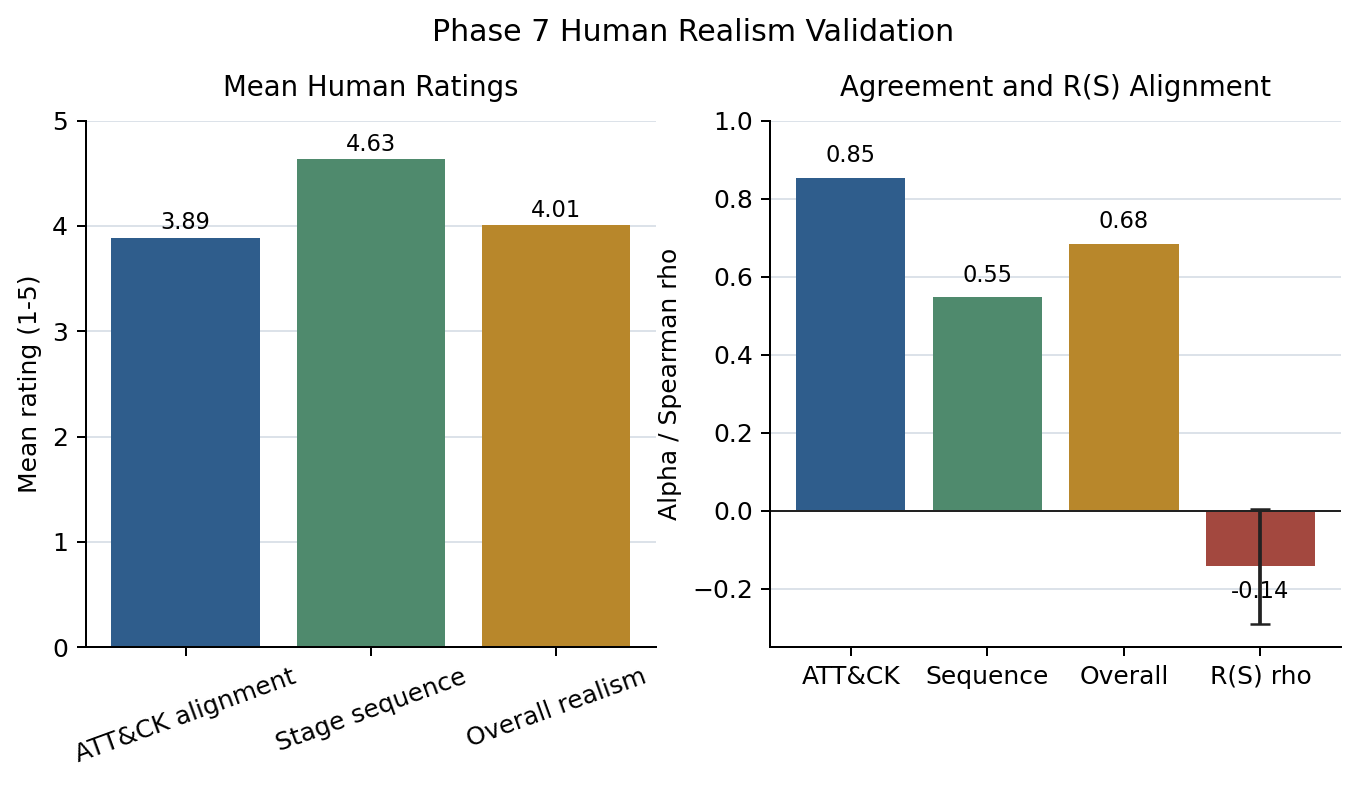
\includegraphics[width=\linewidth]{../paper_assets/figures/phase7_human_validation.png}
  \caption{Human realism validation over \HumanScenarioCount{} blinded
  scenarios rated by \HumanAnnotators{} independent reviewers. Agreement is
  reported using Krippendorff ordinal alpha, while the association between
  $R(S)$ and mean overall human realism is reported separately.}
  \label{fig:phase7}
\end{figure}

\section{Method}

The generation algorithm is a validate-and-requery loop. For each requested
scenario tuple, the system prompts the LLM, parses the response as JSON, checks
required fields, validates ATT\&CK technique identifiers against the active
matrix snapshot, and either accepts the scenario or sends a correction prompt.
The full pseudocode and complexity analysis are provided in
Section~\ref{sec:appendix-methods}.

The structural realism score $R(S)$ combines active-ID validity, attack-stage
and graph structure, and ATT\&CK group transition coherence. Phase~\ref{sec:human}
shows why the paper treats $R(S)$ as a structural consistency metric, not as a
standalone realism oracle.

\section{Results}

\subsection{ATT\&CK Validity and Coverage}

The cleaned corpus contains \ScenarioCount{} scenarios, \UniqueActiveV{} unique
active ATT\&CK techniques, and \UniqueBaseTechniques{} unique base techniques.
This yields \BaseCoverage{} base-technique coverage against the active
Enterprise matrix denominator. Cross-version robustness over
\AttackVersionsCompleted{} ATT\&CK releases preserves a minimum unique-ID active
rate of \AttackVersionMinUniqueActive{} and a minimum per-scenario all-ID
active rate of \AttackVersionMinScenarioActive{}.

\subsection{External Grounding and Real Baselines}

External ATT\&CK transition validation finds \ExtCorrob{} unweighted and
\ExtCorrobWeighted{} weighted transition corroboration, with a Spearman
association of \SpearmanRho{}. A separate third-party report-derived realism
check uses \ExternalReports{} reports and separates real report-derived
sequences from random controls: mean scores are \ExternalRealMean{} versus
\ExternalRandomMean{}, with Cliff's delta \ExternalCliffDelta{}.

Real-system metadata baselines provide a non-author-constructed comparison.
AdverSim covers \BaselineAdverSimBaseCoverage{} of active base techniques with
\BaselineAdverSimTransition{} transition corroboration. CALDERA Stockpile
metadata covers \BaselineCalderaBaseCoverage{} of active base techniques with
\BaselineCalderaTransition{} transition corroboration, while Atomic Red Team
metadata covers \BaselineAtomicBaseCoverage{} of active base techniques but is
single-technique by design.

\begin{figure}[t]
  \centering
  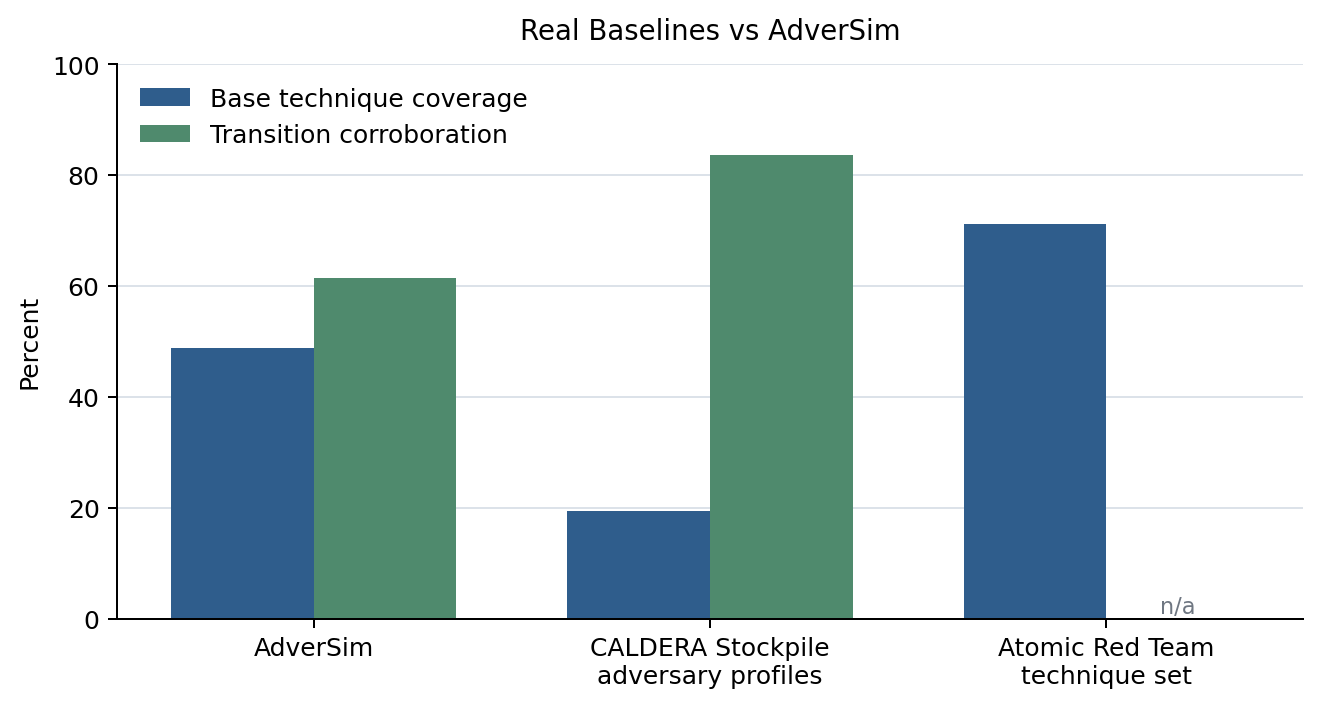
\includegraphics[width=\linewidth]{../paper_assets/figures/real_baselines_coverage.png}
  \caption{Coverage comparison against public real-system metadata baselines.}
  \label{fig:baselines}
\end{figure}

\subsection{Detection Engineering}

AdverSim generates \SigmaRulesGenerated{} Sigma-compatible rule skeletons. In
the replay experiment, \SigmaReplayRules{} generated rules are evaluated over
\SigmaReplayEvents{} labelled events, yielding \SigmaReplayCoverage{} technique
coverage and \SigmaReplayTruePositiveAlerts{} true-positive event alerts. This
result grounds the detection-engineering claim in replayed telemetry while
retaining the limitation that the matcher is intentionally transparent and
keyword based.

\begin{figure}[t]
  \centering
  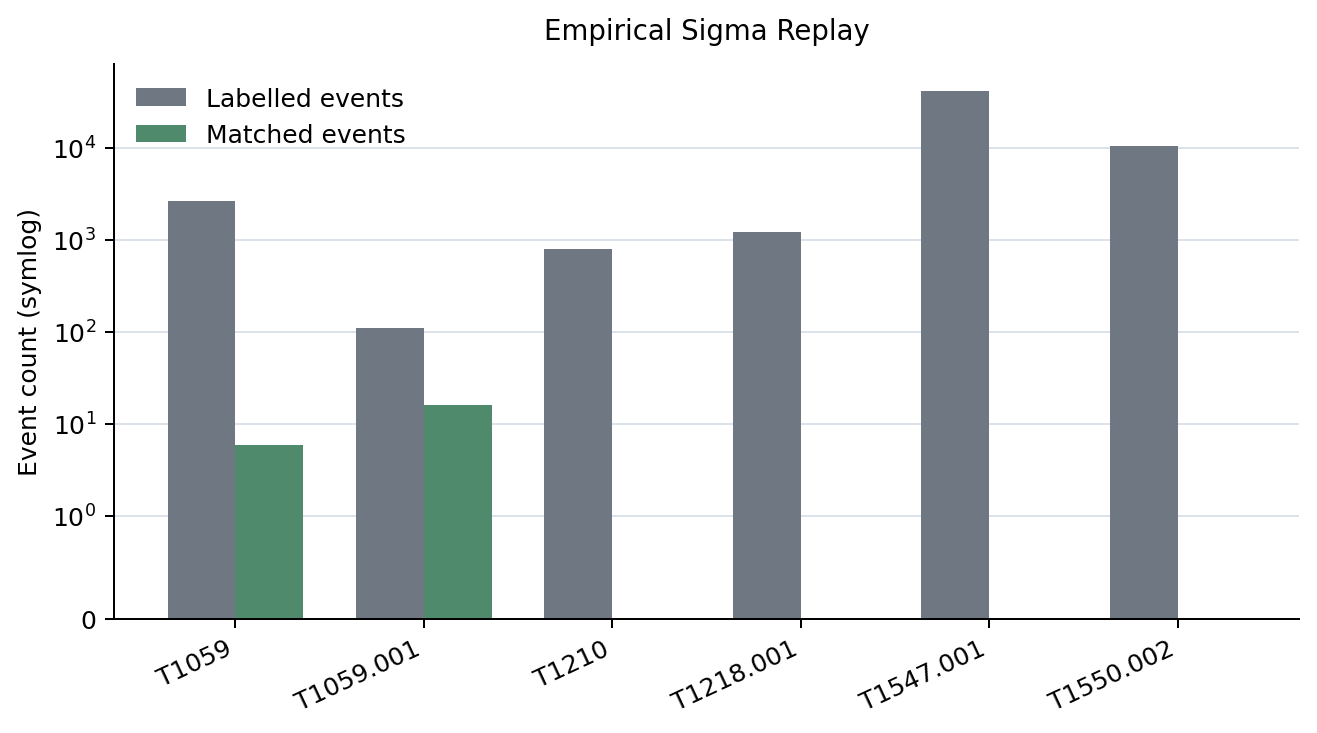
\includegraphics[width=\linewidth]{../paper_assets/figures/sigma_replay_coverage.png}
  \caption{Empirical Sigma replay coverage over labelled defensive events.}
  \label{fig:sigma}
\end{figure}

\subsection{Multi-Model Generalization}

The multi-model replication evaluates \MultiModelsCompleted{} models with
\MultiModelN{} requested scenarios per model. The union contains
\MultiModelUnionActive{} unique active ATT\&CK techniques. First-attempt active
validity is \MultiGptFourOMiniFirstAttempt{} for GPT-4o-mini and
\MultiGptFourOneMiniFirstAttempt{} for GPT-4.1-mini.

\begin{figure}[t]
  \centering
  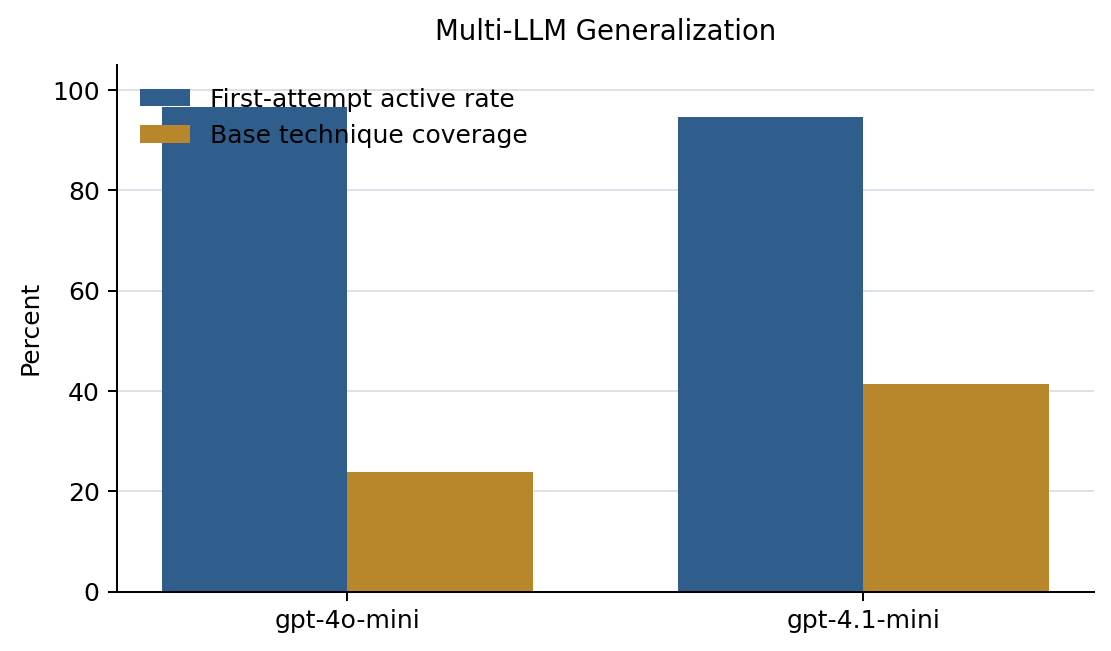
\includegraphics[width=\linewidth]{../paper_assets/figures/multimodel_generalization.png}
  \caption{Exact-size stratified multi-model replication.}
  \label{fig:multimodel}
\end{figure}

\subsection{Human Realism Validation}
\label{sec:human}

Five independent reviewers rated \HumanScenarioCount{} blinded scenarios.
Agreement was strongest for ATT\&CK alignment
($\alpha=\HumanAlphaAttck{}$), moderate for overall realism
($\alpha=\HumanAlphaOverall{}$), and lower for stage-sequence judgments
($\alpha=\HumanAlphaSequence{}$). The association between $R(S)$ and mean human
overall realism was \HumanRsRho{} with bootstrap interval
[\HumanRsCIlo{}, \HumanRsCIhi{}]. This result supports the presentation fix:
$R(S)$ is useful for structural quality control, but human review remains
necessary for realism.

\section{Reproducibility}

All headline values in this draft are macro-wired through
\texttt{paper/generated\_macros.tex}. The repository includes a reproducibility
CI path that regenerates figures, verifies the figure manifest, runs an offline
smoke pipeline, rebuilds the registry, and audits manuscript literals. Fresh
generation remains API-dependent, but figure regeneration and aggregate-result
checks run without API keys or raw logs.

% Table XVI: reproducibility map for the macro-wired manuscript.
\begin{table*}[t]
\centering
\caption{Reproducibility map. Offline checks are separated from API-dependent regeneration.}
\label{tab:reproducibility-map}
\small
\begin{tabular}{p{0.21\linewidth}p{0.24\linewidth}p{0.28\linewidth}p{0.19\linewidth}}
\toprule
Claim family & Command & Primary artifact & Status \\
\midrule
Registry, macros, and figure refresh & \texttt{make reproduce} & \texttt{results/registry.json}, \texttt{paper/generated\_macros.tex}, figures, and manifest & Offline, ready \\
Pre-submission QA & \texttt{make submission-qa} & Reproducibility CI plus repository pre-push checks & Offline, ready \\
Full scale-up corpus & \texttt{make scaleup-full} & Ignored full JSONL corpus, public sample, manifest, and validation summary & API-dependent runnable path \\
Exact-size multi-model replication & \texttt{make multimodel-exact-size} & Per-model ignored corpora plus tracked aggregate table and audit note & API-dependent runnable path \\
Sigma replay grounding & \texttt{make sigma-replay} & Replay coverage and alert summary & Requires labelled event logs \\
Human realism validation & \texttt{make annotation-analyze} & Blinded human-rating aggregate and audit note & Ready with anonymized ratings \\
\bottomrule
\end{tabular}
\end{table*}


\section{Limitations, Ethics, and Safety}

AdverSim scenarios are synthetic. The system is intended for defensive
cyber-range research, teaching, and detection engineering; it does not execute
malware, exploit payloads, Atomic Red Team tests, CALDERA agents, or live
adversary emulation. Raw logs, human rating sheets, reviewer identities, API
keys, and local secrets are excluded from version control.

\section{Conclusion}

AdverSim demonstrates that LLM-generated cyber-range scenarios can be made more
publishable when generation is paired with validation, baselines, human review,
and reproducible presentation. The key presentation change is restraint:
structural consistency, detection replay, and human realism are reported as
distinct evidence streams rather than collapsed into one overbroad realism
claim.

\appendices
\section{Algorithmic Methodology}
\label{sec:appendix-methods}
% Paper-ready methods supplement for AdverSim.
% This file is intentionally package-light. It uses tables and verbatim-style
% pseudocode so it can be pasted into IEEE or ACM templates with minimal edits.

\section{Algorithmic Methodology and Complexity}

Let $N$ be the number of scenarios, $R$ the maximum number of corrective
re-query attempts, $L$ the generated JSON length, $S$ the number of stages in a
scenario, $T$ the number of ATT\&CK technique mentions, $G$ the number of attack
graph edges, $K$ the number of active ATT\&CK techniques, $P$ the number of
ATT\&CK group co-occurrence pairs, $M$ the number of Sigma rules, $E$ the number
of replay events, $H$ the number of human reviewers, and $B$ the number of
bootstrap or permutation resamples. LLM inference dominates wall-clock
generation cost; the local validation and scoring steps are linear in the size
of each generated scenario.

\subsection{System Architecture}

AdverSim is organized as a validate-and-requery generation loop followed by
offline evaluation layers. The generation layer accepts an attack type,
environment, and difficulty tuple, prompts the LLM for structured JSON, parses
the result, validates all ATT\&CK IDs against a fixed active matrix snapshot,
and re-queries when parsing, schema, or technique validation fails. Accepted
scenarios are written to the corpus and then passed to structural scoring,
SOC-simulation sensitivity analysis, Sigma rule generation and replay, real
baseline comparison, blinded human realism validation, and reproducibility CI.

\subsection{Algorithm 1: Validate-and-Requery Scenario Generation}

\begin{verbatim}
Input: parameter tuples X, active ATT&CK set A, max re-query R
Output: accepted corpus C and telemetry Q

C <- empty list
Q <- empty telemetry table

for each x = (attack_type, environment, difficulty) in X:
    prompt <- build_prompt(x)
    accepted <- false

    for attempt in 0..R:
        raw <- call_llm(prompt)
        parsed <- parse_json(raw)

        if parsed is invalid:
            prompt <- correction_prompt(x, "return valid JSON")
            record parse failure in Q
            continue

        issues <- validate_schema_and_attck(parsed, A)

        if issues is empty:
            C.append(parsed)
            record accepted scenario in Q
            accepted <- true
            break

        prompt <- correction_prompt(x, issues)
        record validation failure in Q

    if accepted is false:
        record rejection in Q

return C, Q
\end{verbatim}

The remote generation cost is
$O(N(R+1)\mathrm{LLM}(L))$. The local parsing and validation cost is
$O(N(R+1)(L+T+S+G))$, with local space $O(N(L+T+S+G)+K)$.

\subsection{Algorithm 2: Structural Realism Score}

For a scenario $s$, AdverSim computes active validity, structure, and transition
coherence:

\begin{verbatim}
tids <- ordered ATT&CK IDs from s.attack_stages
active_validity <- count(tid in A for tid in tids) / max(1, len(tids))

structure <- min(1,
    0.6 * len(stages) / 4
  + 0.4 * len(edges) / max(1, len(stages)-1))

transition_pairs <- adjacent unordered pairs from tids
transition_coherence <- count(pair in Pairs for pair in transition_pairs)
                        / max(1, len(transition_pairs))

R(S) <- 0.40 * active_validity
      + 0.35 * structure
      + 0.25 * transition_coherence
\end{verbatim}

Building the group-pair reference set costs $O(\sum_g k_g^2)$ for ATT\&CK
group technique counts $k_g$. Scoring one scenario costs $O(T+S+G)$ and uses
$O(P+T)$ space. The human validation experiment should be used to frame $R(S)$
as a structural consistency metric, not as a complete substitute for human
realism judgment.

\subsection{Algorithm 3: Human Realism Validation}

\begin{verbatim}
sample <- stratified_sample(C, n, attack_type x environment x difficulty)

for each scenario in sample:
    blind_id <- stable hash of seed and sample position
    write blinded scenario row
    write empty reviewer template row
    write hidden key row with R(S) features

collect H completed templates
aggregate ratings by blind_id
compute Krippendorff ordinal alpha by dimension
compute Spearman correlation between R(S) and mean overall realism
bootstrap the correlation confidence interval
fit exploratory R(S) weights on train split and evaluate held-out rows
\end{verbatim}

Packet generation costs $O(N+n(T+S+G))$. Rating aggregation costs $O(Hn)$,
agreement computation costs $O(nH^2)$, and bootstrap correlation costs
$O(Bn\log n)$.

\subsection{Algorithm 4: Detection Engineering and Replay}

\begin{verbatim}
for each selected scenario:
    focus_stage <- first high-signal stage, else first stage
    focus_tid <- first valid technique in focus_stage
    logsource <- map focus_tid to Sigma logsource
    keywords <- technique names and indicator terms
    write Sigma YAML rule

for each labelled event:
    labels <- extract ATT&CK labels
    haystack <- flattened lowercase event text
    for each Sigma rule:
        if logsource is compatible and keyword matches haystack:
            record alert and true-positive status
\end{verbatim}

Rule generation costs $O(M(T+L_s))$, where $L_s$ is stage text length. Replay
with transparent keyword matching costs $O(EMW)$ for average keyword count $W$.

\subsection{Complexity Summary}

\begin{table}[t]
\centering
\caption{AdverSim algorithmic complexity.}
\begin{tabular}{lll}
\hline
Component & Time & Space \\
\hline
Generation & $O(N(R+1)\mathrm{LLM}(L))$ remote & $O(N(L+T+S+G)+K)$ \\
Validation & $O(T+S)$ per scenario & $O(T+K)$ \\
$R(S)$ scoring & $O(\sum_g k_g^2 + N(T+S+G))$ & $O(P+T)$ \\
SOC sensitivity & $O(|\Theta|NS)$ & $O(|\Theta|D+N)$ \\
Sigma generation & $O(M(T+L_s))$ & $O(M)$ \\
Sigma replay & $O(EMW)$ & $O(M+E_{labels}+alerts)$ \\
Human validation & $O(N+n(T+S+G)+Hn+nH^2+Bn\log n)$ & $O(nH+P)$ \\
Figure CI & $O(A+F\cdot pixels)$ & $O(A+F\cdot pixels)$ \\
\hline
\end{tabular}
\end{table}


\section{Validity and Artifact Details}
% Paper-ready validity, ethics, and reproducibility text for AdverSim.
% This section is additive and does not change reported results.

\section{Validity, Ethics, and Reproducibility}

\subsection{Threats to Validity}

\textbf{Construct validity.}
The structural realism score $R(S)$ measures ATT\&CK consistency, scenario
structure, and transition coherence. It should not be interpreted as a complete
proxy for real-world incident realism. The human validation experiment shows
that human overall-realism ratings do not strongly positively align with
$R(S)$, so the metric is best framed as a structural consistency measure that
requires human realism checks.

The SOC simulation is parameterized and should be interpreted as simulation
behavior rather than an empirical production-SOC study. Sensitivity analysis is
therefore used to distinguish invariant findings from model artifacts. Sigma
replay provides defensive grounding by applying generated rule skeletons to
labelled events, but its coverage depends on event availability, label quality,
logsource mapping, and the intentionally transparent keyword matcher.

\textbf{Internal validity.}
The validate-and-requery loop reduces invalid JSON, schema failures, and
inactive ATT\&CK IDs, but it can also bias accepted outputs toward scenarios
that satisfy schema and matrix constraints. Human ratings were collected from
five independent technical reviewers: two software test engineers, one IT
specialist, one master's student in cybersecurity, and one master's student in
computer science. This supports independent human realism checking, but it
should not be described as a panel composed entirely of SOC, DFIR, or
threat-intelligence experts.

\textbf{External validity.}
The corpus covers selected attack types, environments, difficulties, and
ATT\&CK Enterprise techniques. Results may not transfer directly to operational
incidents, non-Enterprise ATT\&CK matrices, highly specialized industrial
control environments, or organizations with different logging maturity. The real
baseline comparison uses public CALDERA Stockpile and Atomic Red Team metadata;
these are useful non-author-constructed baselines but are not complete models of
all real adversary behavior.

\textbf{Statistical conclusion validity.}
Confidence intervals, null models, held-out refits, agreement statistics, and
multiple-testing adjustments are used where the available data support them.
Remaining risks include limited human-reviewer count, aggregate-only legacy
mutation outputs, and correlation estimates that depend on the selected sample
and metric definition.

\subsection{Ethics and Safety}

AdverSim is intended for defensive cyber-range research, teaching,
reproducible evaluation, and detection engineering. The repository generates
structured scenario descriptions and Sigma-compatible detection skeletons. It
does not execute malware, exploit payloads, Atomic Red Team tests, CALDERA
agents, or live adversary emulation. Public baseline scripts parse metadata
only.

Raw defensive logs, raw human rating sheets, reviewer identities, API keys, and
local secrets are excluded from version control. Environment files and key-like
artifacts are ignored, raw annotation directories are ignored, and tracked
outputs contain only aggregate or anonymized results. Out-of-scope uses include
unauthorized intrusion, malware deployment, credential theft, exploit execution,
or evasion testing against systems without authorization.

\subsection{Artifact Availability and Reproducibility}

The repository separates API-dependent generation from offline
reproducibility. The offline path runs without API keys or raw logs: it checks
tracked result artifacts, regenerates paper figures from aggregate outputs,
validates figure hashes through a manifest, runs the smoke pipeline, and scans
for large files or secret-like values. Fresh LLM generation, multi-model
replication reruns, and some public-baseline refreshes are documented separately
because they require API access or network availability.

\begin{table}[t]
\centering
\caption{Methodological components and their role in strengthening validity.}
\begin{tabular}{p{0.23\linewidth}p{0.31\linewidth}p{0.31\linewidth}}
\hline
Component & Contribution & Limitation \\
\hline
Validate-and-requery & Rejects malformed JSON and invalid ATT\&CK IDs before corpus acceptance & Does not guarantee full tactical realism \\
Single ATT\&CK source of truth & Makes technique counts traceable to one matrix snapshot & Depends on selected ATT\&CK version \\
Cross-version robustness & Tests behavior under v13/v14/v15 matrix drift & Limited to Enterprise ATT\&CK \\
Statistical rigor & Adds confidence intervals, null models, and effect-size framing & Some legacy outputs remain aggregate-only \\
SOC sensitivity & Separates invariant findings from model artifacts & Not a production-SOC study \\
Sigma replay & Grounds detection claims in labelled events & Depends on labels and simple matching \\
Real baselines & Compares against public non-author-constructed metadata & Public corpora are heterogeneous \\
Human validation & De-biases $R(S)$ with blinded human ratings & Reviewers are technical, not all SOC/DFIR experts \\
Reproducibility CI & Regenerates figures and verifies artifacts without secrets & Fresh generation still requires API access \\
\hline
\end{tabular}
\end{table}

\subsection{Data and Model Card Summary}

\begin{table}[t]
\centering
\caption{AdverSim data and model card summary.}
\begin{tabular}{p{0.32\linewidth}p{0.56\linewidth}}
\hline
Field & Summary \\
\hline
Artifact & Synthetic cyber-range scenario corpus in JSONL format \\
Scenario structure & Narrative, environment, difficulty, attack type, stages, ATT\&CK techniques, and attack graph \\
Main ATT\&CK matrix & Enterprise v14.1 active-technique index \\
Robustness checks & Additional v13/v14/v15 validation audit \\
Human validation & 150 blinded scenarios rated by five independent reviewers \\
Reviewer composition & Two software test engineers, one IT specialist, one MSc cybersecurity student, one MSc computer science student \\
Raw sensitive files & API keys, raw logs, raw rating sheets, and reviewer identities excluded from git \\
Intended uses & Cyber-range scenario generation, defensive evaluation, teaching, and reproducible research \\
Out-of-scope uses & Unauthorized intrusion, exploit execution, malware deployment, credential theft, or unsanctioned evasion testing \\
\hline
\end{tabular}
\end{table}

\subsection{Limitations Statement}

AdverSim scenarios are synthetic and should not be interpreted as substitutes
for real incident reports or telemetry. The validation pipeline reduces
malformed outputs and invalid ATT\&CK IDs, but tactical realism remains partly a
human judgment. Accordingly, $R(S)$ is reported as a structural consistency
metric, while blinded human ratings provide an independent realism check. SOC
detection results are presented as simulation and sensitivity-analysis outputs,
not as measurements of analyst performance in a production SOC.


\end{document}
